\chapter{Literature Survey}

The development of Wireless Sensor Network (WSN) is considered to be one of the greatest innovation in the field of electronics. The miniaturization of the components has allowed exploration of applications in various fields such as health care, military applications, traffic control, monitoring, and data collection \cite{Khedo2017} \cite{Liu2017}. Out of all the applications, urban air quality monitoring has gained a lot of attention as it is one of the major issues faced by society today. While reviewing the related work, we found that there are various methods that can be used to understand pollution. These could be classified into three based on literature as follows \cite{Yi2015} \cite{Pavani2017}.




%There are different approaches for measuring air pollution and this chapter gives an overview of the research work done for understanding this based on the medium for measurement. The popular mediums used for the measurement can be classified as below
 
\begin{enumerate}

    \item Vehicle-based sensor network
 %   \item Wearable sensor network
    \item Community sensor network
    \item Static sensor network

 \end{enumerate} 

 Further, we will be highlighting the important research done in each of the above four categories and will be classifying to which category our work falls.

\section{Vehicle based sensor network (VSN)}

In recent times, the number of private vehicles on the road has increased in proportion to the increasing population around the globe \cite{Downs2004}. Even though the increase in the number of automobiles is one of the major factors that is contributing to the increase in pollution, certain researchers took this as a medium for measuring air pollution data. In this category of work, the vehicles (like buses or cars) are installed with a portable, low-cost sensor to obtain spatially resolved data. 
\par
%Portable and low-cost sensors are installed and attached to a vehicle like buses or cars in order to achieve a spatially resolved data. There have been an increasing number of mobile vehicles in urban areas. This was taken as a medium for obtaining air pollution data from the environment in cities. 
 One of the best ways to study the air quality is by collecting fine-grained data also called \lq{micro-climate monitoring}\rq. However, since the existing monitoring systems are bulky and expensive it is impossible to obtain spatially resolved data. To solve this issue, in 2009 a group of researchers used mobile monitoring as a method and proposed a vehicular wireless sensor network \cite{Hu2009} that measures the changes in concentration of a single pollutant (Carbon Dioxide in this case) by mounting the sensor node onto a vehicle. The system is equipped with a Carbon Dioxide ($CO_2$) sensor, a Global System for Mobile (GSM) module, a GPS receiver, and a ZigBee module to create an intra-vehicular network. The collected data is transferred through GSM short messages to the server and is displayed on Google Maps for results. The architecture of the VSN is shown in the figure\ref{vsn}. 

 \begin{figure}[h!]
  \begin{center}
  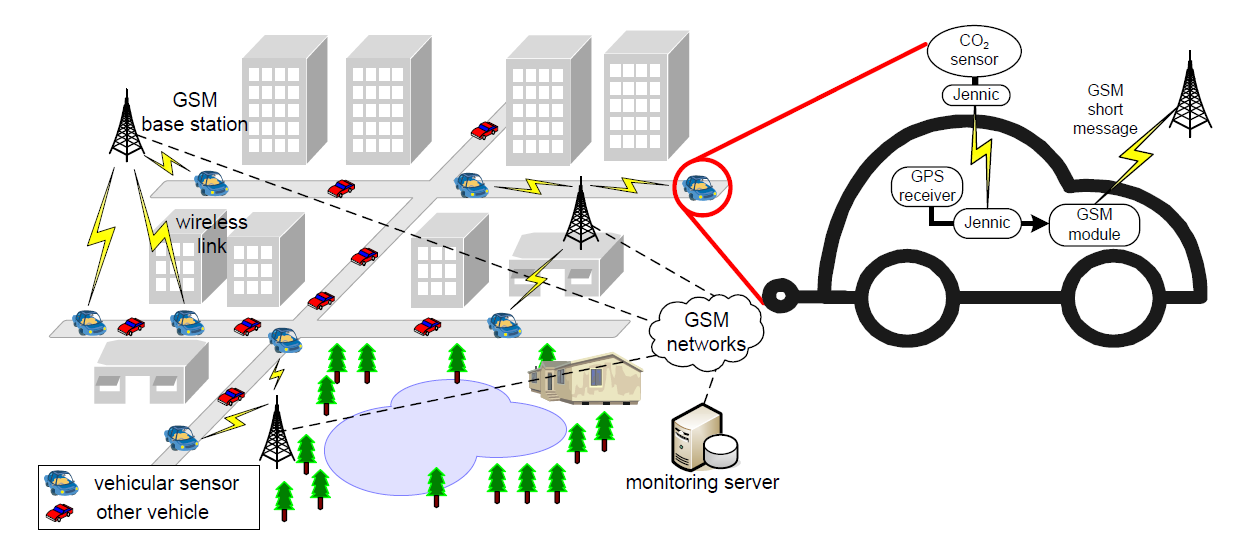
\includegraphics[scale=0.65]{./images/figure40.png}
  \end{center}
 
  \caption{Architecture of Vehicular based sensor network \cite{Hu2009}}
  
  \label{vsn}
\end{figure}
 
 This work faced two network-related drawbacks. Firstly there was a duplication of air pollution data as the number of vehicles in a given area changed dramatically from time to time and secondly, to reduce the data transfer in an area with many sensor nodes at the same time by exploiting opportunistic communication. These two problems were later addressed in 2011 by designing two message-efficient algorithms \cite{Hu2011}. The first algorithm works by dividing the sensing field into a fixed number of grids and each grid was allocated with a particular reporting rate which is called dynamic reporting rate to reduce communication overhead. The second algorithm allows the sensing nodes to communicate with each other and find out their reporting rate and opportunistically transfers the collected data. %The main area of the work revolved around data collection, optimization of the collected data, and concentrating only on one pollutant. The other issues like the quality and accuracy of the collected data, management and operations of wireless sensor networks were not given priority.

 %They also created a simulation model to verify the performance of the algorithm. The above two research work mainly focused on data collection, optimization of the collected data, and only revolved around one pollutant. The problems like calibration of sensors, visualization of data, checking the accuracy of the collected data, and management of the VSN was not taken care of.

 %Volgyesi et al. \cite{Volgyesi2008} proposed the Mobile Air Quality Monitoring Network (MAQUMON) that measured three pollutants, Ozone ($O_3$), Carbon Monoxide ($CO$), and Nitrogen Dioxide ($NO_2$). The air pollution system is mounted on a car and is powered by a Li-ion battery whose battery life is limited to a few hours. It is equipped with a GPS module for determining the location and the collected data is transferred to a laptop through a Bluetooth module. When the system is in coverage of a Wi-Fi network the collected data is transferred to a web server and visualized in sensor map web application in the form of contour maps. %However, the inability of representing instantaneous data is one of the main concerns with this system and also have failed to show the accuracy of collected data to the local system.


\par

The next work discussed below involves data collection that requires more frequent and spatially dense pollutant measurement and is called a fine-grained approach. In the reference paper \cite{Devarakonda2013}, the vehicular-based approach of measuring
fine-grained air quality in real-time was demonstrated. To increase the spatial density, the study proposed two cost-effective data collection models: one for public transportation infrastructure and the other for a personal sensing device. In the public transportation infrastructure model, a Mobile Sensing Box (MSB) was installed in public transit buses which contained the microcontroller (Arduino), sensors for measuring Particulate Matter ($PM$), and Carbon Monoxide ($CO$), a GPS module, and a cellular modem. The module was powered through the bus batteries and the collected data were transferred to a server and visualized in a platform called Google Fusion tables interfaces. In the other data collection model, a Personal Sensing Device (PSD) that included an air quality sensor was installed in cars and connected via Bluetooth to a smartphone. This gave the user information about the air quality while driving through a specific area.
The data obtained from both the models were compared using linear regression and the results showed a positive linear relationship between the data sets. These collected data were available to the public through customized web and mobile Apps. %Even though there was a high correlation seen between the two sets of data there was no comparison with the local reference data to understand the accuracy of the system.

\par
%Another fine-grained approach of data collection can be seen in an IoT based air quality monitoring using a wireless sensor deployment \cite{Saha2017} that proposed the idea of placing the sensor nodes in public transport buses to obtain real-time data of pollutants. This system is divided into a sensor node and a sink node in which the former collects the data from the environment and the latter aggregates the data from the sensor node and transmits it to a server via a long-range radio band. These sink nodes are installed at a T-junctions or X-junction of the city where most of the buses cross. The data is transferred at a regular interval to a cloud server and analyzed. %However, the paper did not discuss the collection of data and failed to provide the quality of collected data.



A research group from Japan, Shirai et.al \cite{Shirai2016} proposed an effective method to acquire air quality data in urban areas in which the air pollution system has a sensing unit mounted on a public vehicle such as a garbage truck that moves in and around the city. The main focus is on pollutants like Particulate Matter ($PM$), Carbon Monoxide ($CO$), and Sulphur Dioxide ($SO_2$). The system is also equipped with a GPS module to identify the location. A control centre tool was developed to check for maintenance and remotely control the sensor system. The control centre consists of a map that tracks the route of the vehicles and the sensor data acquired by each vehicle. A monitor was developed along with the system to send the users (which in this case is the local citizens in Fujisawa City, Japan) the collected data. The system estimates the amount of pollution inhaled by the user by acquiring the user's location from the mobile application and mapping it to the location-sensors value which has been already computed.

Another mode of transportation that has been used to understand the air quality was the public bicycle system. The bicycle-borne sensor \cite{Xiang2016,Liu2015a} system consists of an exhaust gas sensor, Particulate Matter ($PM$) sensor, GPS module, Bluetooth module, and a microprocessor. The system collects pollutant data along with the location data from the GPS module and is stored in a storage chip. When the subscriber returns the bicycle to the dock station, the data is transferred to the data center via the Bluetooth module and is then visualized using the \lq{Baidu}\rq heat map (similar to Google maps that are used in China).


 Unmanned Aerial Vehicle (UAV)  that do not need on board human pilot are also used to understand air quality \cite{Zhi2017}. This work focused on six different pollutants that contribute to Air Quality Index by mounting the sensor board on the UAV. The flights were carried out for 30 days with 20 minutes of monitoring. Along with the sensor board, a smartphone is attached that collects data from the air sensors by establishing a Bluetooth connection. The collected data is transferred to air quality analysis software that will display the real-time monitoring value along with AQI value. 

The previous studies in this section show that collecting data using VSN can support micro-climate monitoring. The advantage of having spatially resolved data is that it helps to understand the local trends of pollution. Having high mobility of sensor nodes helps to cover a larger geographic area and gives access to data in the areas where the reference system is not available. However, the majority of work only focused on data collection and optimization of data. The main idea of deploying any system for measuring air pollution is to educate citizens and make them aware of air quality through the indices. The efforts to calculate AQI or AQHI was not in the studies described above. The communication of these indexes will make people aware of the air quality, but most of the work to date in this category has failed to bridge the data gap.


%\section{Wearable sensor network (WSN)}


%The effect of pollutants on the health of an individual depends on the extent to which that person is exposed to the polluted environment. The understanding of the health effects could be achieved by the amount of pollutants inhaled by an individual observing the exposure-response relationship \cite{Dons2017}. This could be achieved by using a wearable sensor system that measures exposure to polluted air. Research work done in this section mainly focuses on improving the understanding of exposure to air pollution and personal health \cite{Hu2015}. One such development is \lq{Mypart}\rq \cite{Tian2016} which is a wrist-worn particle sensor that measures particulate matter of 10 microns or less ($PM_{10}$). The design of MyPart is based on a laser-based photodiode system with integration of structural design and circuitry for ambient visualization, BLE transceiver for low power networking, and also a mobile application for visualization.The two main issues tackled by MyPart are accuracy and calibration of the sensor which no existing consumer sensor had addressed.

%Another work in WSN is \lq{Eco-mini}\rq \cite{Fletcher2015} which is a wearable stand-alone device for clinical use that measures Ozone, Sulphur
%Dioxide, Volatile Organic Compounds (VOCs), sound level, temperature, and humidity values. This system is based on a low power microcontroller (Atmel Xmega 128k) and consists of a GPS module for location and a Bluetooth module for data transfer. They developed and webserver and a mobile application for data visualization. The next wearable work is \lq{CitiSense}\rq \cite{Zappi2012} which is a system attached to a bag stripe which measures the air pollutants Nitrogen Dioxide ($NO_2$), Carbon Monoxide ($CO$), and Ozone  ($O_3$) along with environmental parameters such as temperature, humidity, and barometric pressure. The collected data from the sensor is processed by a microcontroller (ATMEGA1284p) and transfers the data using a Bluetooth module to a smartphone which does the data storage, analysis, and data aggregation. The collected data is then transferred to a back-end webserver from where the user can get a personalized view of their data.
 
%A group of researchers from US developed an expressive T-shirt called \lq{WearAir}\rq \cite{Kim2010} which indicates the measured Volatile Organic Compounds (VOC) through expressive patterns. The T-shirt display is designed with the metaphor of a car emitting gases using four vertical arrays of LEDs which displays different flash frequencies depending on the concentration of VOC gas detected. When the wearer is exposed to dense VOCs the LED arrays will blink rapidly. 
%The authors of \cite{Hu2014} developed a novel system consisting of several sensors that give real-time feedback on an individual's exposure dose. This consist of arm sensors, chest sensor or even wrist sensors which measures various pollutant concentration ($CO$ in this case) and transfers to an android or ios application via Bluetooth. They also calculate the inhaled dose of pollutants by calculating the volume of air inhaled into a person's lung per minute through an algorithm developed in \cite{Valli2013}. The inhaled dose of the pollutant was calculated and compared during various activities like jogging, bicycling, and driving.

 %There are also wearable sensor projects initiated in Vancouver in association with the University of British Columbia such as TZOA \cite{tzoa} that can be clipped to the clothing and measures $PM$ values and display in an application. These devices decrease the gap between individual and their awareness of polluted air in their local environment. In NewYork a project named \lq{Aircasting}\rq \cite{aircasting} provides the health and environment data to the users with the help of the android \lq{Aircasting app}\rq. The \lq{Aircasting}\rq\cite{Han2010} platform includes a palm-sized monitor that measures $PM_{2.5}$, relative humidity, and temperature. The outside air is drawn through a sensing chamber and the particles are measured through the light scattering method. It also includes an LED wearable apparel named \lq{Air casting luminescence}\rq \cite{Luminescence} that illuminates LEDs according to the real-time sensor measurement; varying from red for high intensity, then orange, then yellow, and finally green for low intensity. 

 %The above studies in this section give an idea about a different method of data collection. Most of these devices remain unknown to the public and the majority of them do not prefer to wear T-shirts to carry a device for understanding pollution. Another issue to be focused on is the cost which lowers the interests of the public.



\section{Community sensor network (CSN)}



Technological development has paved way for a novel paradigm known as crowdsourcing. Crowdsourcing involves collecting information from a large group of people through the internet or other means and utilizing the collected information towards a common goal. In a community sensor network the use of crowdsourcing or participatory sensing is achieved with the help of a portable sensor network. This allows any citizen to collect data and transfer it to a common platform like a web interface. Various research work falls under this category.
%The development of portable sensor devices has paved way for a novel paradigm for monitoring pollution known as crowdsourcing or participatory sensing. Crowdsourcing involves collecting information from a large group of people. This allows any citizen to collect data and transfer it to a common platform like a web interface. In the study of air pollution crowdsourcing has played a significant role and many research works fall under this category.In this case, the collected data from participants can give a spatiotemporal view of the effect of pollution \cite{Kanhere2013}.
 
 %In Sydney, a low-cost participatory system is deployed named 'Haze-watch' \cite{Sivaraman2013} for monitoring pollution in urban areas. In this system, mobile sensor units were attached to vehicles, and the data collected was transferred using Bluetooth to a mobile application which tags its location with date and time information. This data is then sent to a cloud-based server that stores the data and applies interpolation models \cite{Liao2006} to generate spatio-temporal estimates. A web application is used to visualize the geo-referenced data that is depicted as a contour map. 


 \par
One of the popular methods to achieve CSN is through mobile participatory sensing in which individuals carry portable handheld devices that measures the pollutants. Intel has developed a prototype system named \lq{Common Sense}\rq \cite{Dutta2009} which is based on mobile participatory sensing that enables citizens to collect pollutant data. The system includes a handheld device that measures several pollutants (example: Carbon Monoxide ($CO$), Nitrogen Oxide ($NO$), Ozone ($O_{3}$), temperature, and humidity) and uploads the data using Bluetooth or GPRS radios for visualization over the web. This system was further tested by deploying it on a municipal fleet of street sweepers in the city of San Francisco \cite{Aoki2008}. 

The next portable and crowdsourced monitoring system on list is \lq{Mypart}\rq \cite{Tian2016} which is a wrist-worn particle sensor that measures particulate matter of 10 microns or less ($PM_{10}$). The design of MyPart is based on a laser-based photodiode system with integration of structural design and circuitry for effective visualization, BLE transceiver for low power networking, and also a mobile application for visualization.The two main issues tackled by MyPart are accuracy and calibration of the sensor, which no existing consumer sensor had addressed.



Another participatory-driven sensing system is \lq{Eco-mini}\rq \cite{Fletcher2015} which also a wearable stand-alone device for clinical use that measures Ozone ($O_{3}$), Sulphur Dioxide ($SO_{2}$), Volatile Organic Compounds (VOCs), sound level, temperature, and humidity values. This system is based on a low power microcontroller and consists of a GPS module for location and a Bluetooth module for data transfer. They developed  webserver and a mobile application for data visualization. The next wearable work is \lq{CitiSense}\rq \cite{Zappi2012} which is a system attached to a bag stripe which measures the air pollutants Nitrogen Dioxide ($NO_{2}$), Carbon Monoxide ($CO$), and Ozone  ($O_{3}$) along with environmental parameters such as temperature, humidity, and barometric pressure. The collected data from the sensor is processed by a microcontroller and transfers the data using a Bluetooth module to a smartphone which does the data storage, analysis, and data aggregation. The collected data is then transferred to a back-end webserver from where the user can get a personalized view of their data.




\begin{figure}[h!]
  \begin{center}
  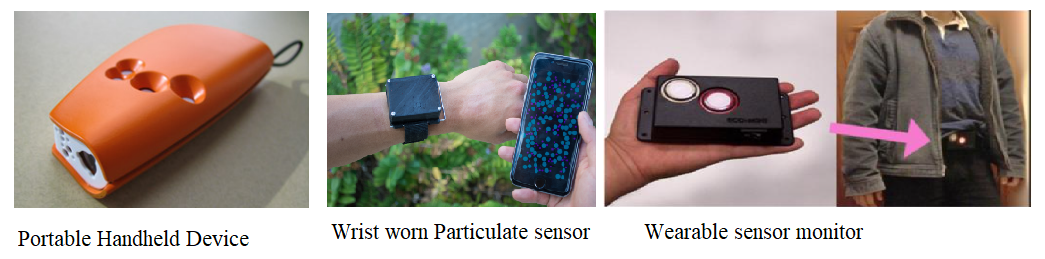
\includegraphics[scale=0.80]{./images/figure41.png}
  \end{center}
 
  \caption{Examples of Community Sensor Network \cite{Tian2016}, \cite{Dutta2009}, \cite{Fletcher2015} }
  
  \label{CSN}
\end{figure}
 
%Another group of researchers also developed an expressive T-shirt called \lq{WearAir}\rq \cite{Kim2010} which indicates the measured Volatile Organic Compounds (VOC) through expressive patterns. The T-shirt display is designed with the metaphor of a car emitting gases using four vertical arrays of LEDs which displays different flash frequencies depending on the concentration of VOC gas detected. When the wearer is exposed to dense VOCs the LED arrays will blink rapidly. 

There are also crowdsourced projects initiated in Vancouver such as TZOA \cite{tzoa} that can be clipped to the clothing and measures $PM$ values and displays this in an application. These devices decrease the gap between individual and their awareness of polluted air in their local environment. In NewYork a project named \lq{Aircasting}\rq \cite{aircasting} provides the health and environment data to the users with the help of the Android \lq{Aircasting app}\rq. The \lq{Aircasting}\rq\cite{Han2010} platform includes a palm-sized monitor that measures $PM_{2.5}$, relative humidity, and temperature. Outside air is drawn through a sensing chamber and the particles are measured through the light scattering method. It also includes an LED wearable apparel named \lq{Air casting Luminescence}\rq \cite{Luminescence} that illuminates LEDs according to the real-time sensor measurement; varying from red for high intensity, then orange, then yellow, and finally green for low intensity. 

The wide availability of the Micro-Electro-Mechanical System (MEMS) and Wireless Sensor Network (WSN) have changed how physical world collect data and interpret them. \lq{G-Sense}\rq \cite{Perez2010}, for Global-Sense, is an initiative from the University of Florida in which they combine features of sensing platform applications like Location-Based Services (LBS) for tracking and location identification, Participatory Sensing (PS) for determining pollution index, and other environmental data, and Human-Centric Sensing (HCS) for health-related data for a specific group of users. The sensors collect data and send it to a first-level integrator where all the data is combined and then a data transport network transfers the data to the server that stores and performs data processing. The data visualization takes place from the server. Later another system which is considered to be the subset of \lq{G-Sense}\rq and was named as 'P-Sense' \cite{Mendez2011} or Pollution-Sense. The architecture of this system is based on \lq{G-Sense}\rq in which external sensors are integrated using an Arduino development board. In this system the data collection is based on Participatory Sensing (PS) and the goal is to provide government officials, doctors, and community developers with data so as to get a deeper understanding. They have also pointed out the research and implementation challenges that need to be addressed when building a community networked system in considering issue such as security, privacy, and data visualization.

The work discussed in this category seems to be promising but at the same time the quality of data obtained, getting public involvement for data collection, and privacy issues \cite{Yi2015} are a few of the challenges researchers are trying to deal with. The cost of maintenance of such a community network is also a crucial factor.


%Another community-driven sensing system that has been developed is \lq{OpenSense}\rq \cite{Aberer2010} which focuses on the utility of data by giving an idea about how the data collected from sensors needs to be consumed. They have provided two use-cases first one is smart healthcare which by giving alerts on identifying the pollution-induced diseases (like asthma, particle allergies, etc.) and next is urban planning by identifying polluted areas and identifying alternative routes. The system is deployed on mobile vehicles and stationary stations in Switzerland and the collected data is pipelined to a Global Sensor Network (GSN) from where the streamed data is processed and represented.


%Another community-driven sensing system that has been developed is \lq{GasMobile}\rq \cite{Hasenfratz2012} which is an outdoor participatory monitor by connecting a low-cost ozone sensor to an android smartphone. The collected data from the sensor is transferred to the phone and from which it is visualized using an application as well as a webserver. They have also implemented calibration procedures to the low-cost sensors and the work claims to have high accuracy when compared to static measurement. The above-mentioned research work in 'OpenSense' and 'GasMobile' have made an opening for further participatory sensing research in Switzerland supported by Samsung called 'Exposuresense' \cite{Predic2013} that monitors user activities like walking, running, etc., from smartphones and understanding their exposure from obtaining data from the already installed 'OpenSense' and 'GasMobile'. Their main idea here is to make use of the available smartphone for next-generation healthcare.


\section{Static sensor network}

 In this category, the system is kept at a fixed location (example: traffic lights, street lights) or any planned areas \cite{Pavani2017} which collects the pollutant values and transfers the data to a visualization platform where the users can view it. These systems are designed to be  inexpensive and so can be easily replicated or replaced. The system can be used for measuring either indoor or outdoor pollutants. There is a variety of research work done under this category and here I reviewed few relevant ones.
 \par
  A research group from Hong Kong developed an Integrated Environmental Monitoring System (IEMS)\cite{Wong2014} that integrates different environmental detection sensors ($PM_{2.5}$, UV sensor, noise sensor, temperature and humidity sensor) into a single system, and data from this system is used for processing and visualization. IEMS consists of Integrated Environmental Monitoring Devices (IEMD) which combine microcontroller units, sensors, and wireless communication modules. The research group also developed a Handheld Remote Control Panel (RCP) for the system which is an Android application that acts as an interface for the device control and handles the data exchange between IEMD and web server. Finally, the webserver provides real-time data visualization and data analysis. These systems were placed at bus stops, bridges, and even at construction sites. 
  
  Another research team from Mauritius developed a Wireless sensor network Air Pollution Monitoring System (WAPMS) \cite{K.Khedo2010} that utilized a data regression algorithm called Recursive Converging Quartiles (RCQ) to remove duplicate data and then calculate AQI values. The array of sensor nodes collects the pollutant data and transfers it to cluster heads where the RCQ is applied to improve efficiency and alleviate the congestion problem. From the cluster head, the data is sent to the server and represented (using line graphs for each area).

'AirSense'\cite{Fang2016} is an approach to assess indoor air quality. This research work introduces the idea of indoor air quality by proposing a system which measures indoor pollutants. The system works through electronic sensors that are coupled to an Arduino microcontroller. The system not only extracts the data but also provides its users with effective visualization and analysis of the data. The researchers have developed this system to sense pollution and provide education and awareness among its users. This system made use of machine learning algorithms to predict the pollution sources and forecast their behaviour that in turn increases the predictive intelligence of the system. The system also uses a smartphone application that gives users an interface for visualization and interpretation of the data. 


\begin{figure}[h!]
  \begin{center}
  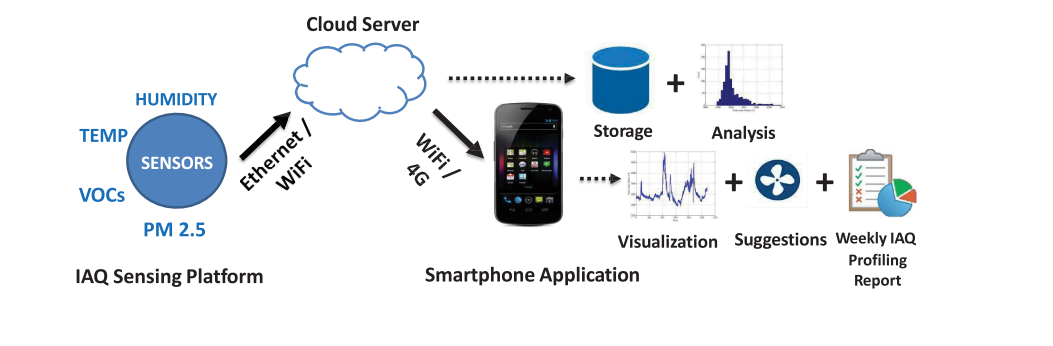
\includegraphics[scale=0.80]{./images/figure42.png}
  \end{center}
 
  \caption{Architecture of a Static Sensor Network (SSN) - AirSense \cite{Fang2016} }
  
  \label{CSN}
\end{figure}



A different group of researchers from China also developed the system 'Air-Sense' \cite{Liu2017} to monitor and predict the quality of air using the ZigBee network to connect the sensors. The system uses four different types of sensors: humidity, temperature, $PM_{2.5}$, and Total Volatile Organic Compound (TVOC includes the general organic gases). A ZigBee trans-receiver is used for communication with network nodes. This prototype is tested in different areas in the house.
\par

Another static system that focuses on indoor air quality in which the main focus is to understand the pollution in an office environment where the pollution is triggered by electronic devices and machines \cite{Firdhous2017}. In this, the pollutant measured is ozone, which is mainly emitted from a photocopier machines. The system is designed with different nodes where the sensing node contains the Arduino microcontroller which collects the data from the ozone sensor. The measured data is transferred through a Bluetooth link to a gateway node from where the data is forwarded over the Ethernet network to the processing node. The data is saved in a database and using a 2D graph the concentration gets visualized. A research group from Harvard University developed a wireless networking testbed called as 'CitySense' \cite{Murty2008} in which multiple environmental sensors are attached to street lights. These sensors were deployed in Cambridge MA and data was uploaded to a server using mesh networks like RoofNet \cite{Bicket2005}, TFA \cite{Camp2006}, and CUWin \cite{cuwin2006}. Using a web-based interface the data can be pulled from the server and made available to end-users. The main feature of this system is that the sensor nodes are powered from street lights and there is no constraint from battery life.
\par
Liu et al \cite{Liu2011} developed a micro-scaled air quality monitoring system for understanding the $CO$ emissions from vehicles by integrating the sensor nodes with a network gateway. The data collected from the sensor is transferred to the gateway using a ZigBee communication link and from here meteorological data and collected sensor data are forwarded to a central system through GSM. This centralized control system is supervised by a LabVIEW \cite{INSTRUMENTS2013} program which helps in store the data into a MySQL database. They deployed the system on the main roads of Taipei (Taiwan) and obtained accurate values of pollutant concentration.


 \section{Summary}


 In this chapter, we discussed the relevant works done in measuring the air pollutants using sensor networks. The work can be categorized mainly into three on the basis of carriers of the sensor node which are vehicle-based, community-based, and static sensor network. There has been a lot of research work done in each category and efforts are made to understand the air pollution by building a system and deploying it on a buildings, vehicle or by crowdsourcing. Our research project falls under a static sensor network category in which we have tried to integrate a system that measures the major pollutants in the city of Prince George and also provide AQHI values. Unlike the other systems mentioned in the literature, our main focus is to give  user-specific data by categorizing the users into three; layman, data scientist and the public officials. We have also tried to implement a calibration procedure to ensure the quality of data. In next chapter, we will discuss the system design and its working. 
 %We went through the system which is attached to a vehicle for understanding the pollutant concentration and gets categorized as a vehicular sensor network. This category provides great mobility but at the same time, the accumulation of redundant data is high.
 %The next category we mentioned is the sensors that could be worn or attached to a person. This gives a better understanding of the individual health effects of the pollutant and also the amount of pollutant inhaled. The work under this category has not gained a lot of attention as it demands the individual to carry the device. 
%Participatory sensing is the next category in which the citizens perform the collection of data and it gets transferred to a common platform. Although the work done in this is more promising it faces challenges like privacy, data quality, and maintenance cost. The final category is in which the system is placed at a planned area and called as a static sensor network. Our research work falls under this section and we focus not just on collecting pollutant value but also on making an effective visualization to reduce the data gap for users.